%!TEX root = thesis.tex

\chapter{Introduction and Overview}
\label{chp:Intro}
In this section, you find a basic introduction to the template. We cover different topics of \LaTeX\ to demonstrate, how your text looks like. For this, we introduce some text and further elements, such as figures and special environments. This section aims at introducing the basic \LaTeX\ elements. Handling and configuring the template is handled in the next section.

\section{Laying the Foundations}
\label{sec:1:LaTeX}
To use this template, you need a \LaTeX\ installation. Yes, there are options to use \LaTeX\ online, e.g., Overleaf, however, I strongly suggest you installing a \LaTeX\ distribution locally. Why? Overleaf is an online platform, i.e., you need a permanent Internet connection to use it. Also, there is \textbf{no guarantee} that this thesis template works with Overleaf, since it configures and handles several aspects automatically. So, my recommendation is to use a local distribution.

\paragraph*{Windows Installation}
Depending on the actual platform that you use, there are different options. The standard solution for Windows users is the \emph{MikTeX} environment, which can be found here: \url{https://miktex.org} (last access: 2024-09-23). Even though the project page tells you that you can minimize the footprint, you should ignore this promise and you should go for the full distribution as, otherwise, you will have to go through several update and installation procedures when first compiling your document. To work with \LaTeX, you also need an editor. Again, for Windows, \emph{TEXnicCenter} (\url{https://www.texniccenter.org}, last access: 2024-09-23) is a good choice. If you use this tool, ensure that you have installed \emph{MikTeX} fist so that \emph{TEXnicCenter} can perform the configuration automatically.

\paragraph*{Mac Installation}
For Mac users, the recommendation is the \emph{TeX Live} distribution (\url{https://www.tug.org/texlive}, last access: 2024-09-23). Please note that this distribution is also available for Windows and Linux. The advantage of this distribution is that it already comes with the basic, required tools like editors and literature management. For instance, the template document that you are reading just now has been created with \emph{TeX Live} on a Mac using \emph{TeXShop} (cf.\ Figure~\ref{fig:texshop}) and \emph{BibDesk}---tools that are included with the \emph{TeX Live} distribution. Same as for \emph{MikTeX}, I strongly suggest installing the full distribution and to run the update procedures (\emph{TeX Live Utility}, just start and let it run) immediately. Also, from time to time, you should run the updates as the \LaTeX\ community is continuously working on the packages' quality.
\begin{figure}[htbp]
	\centering
	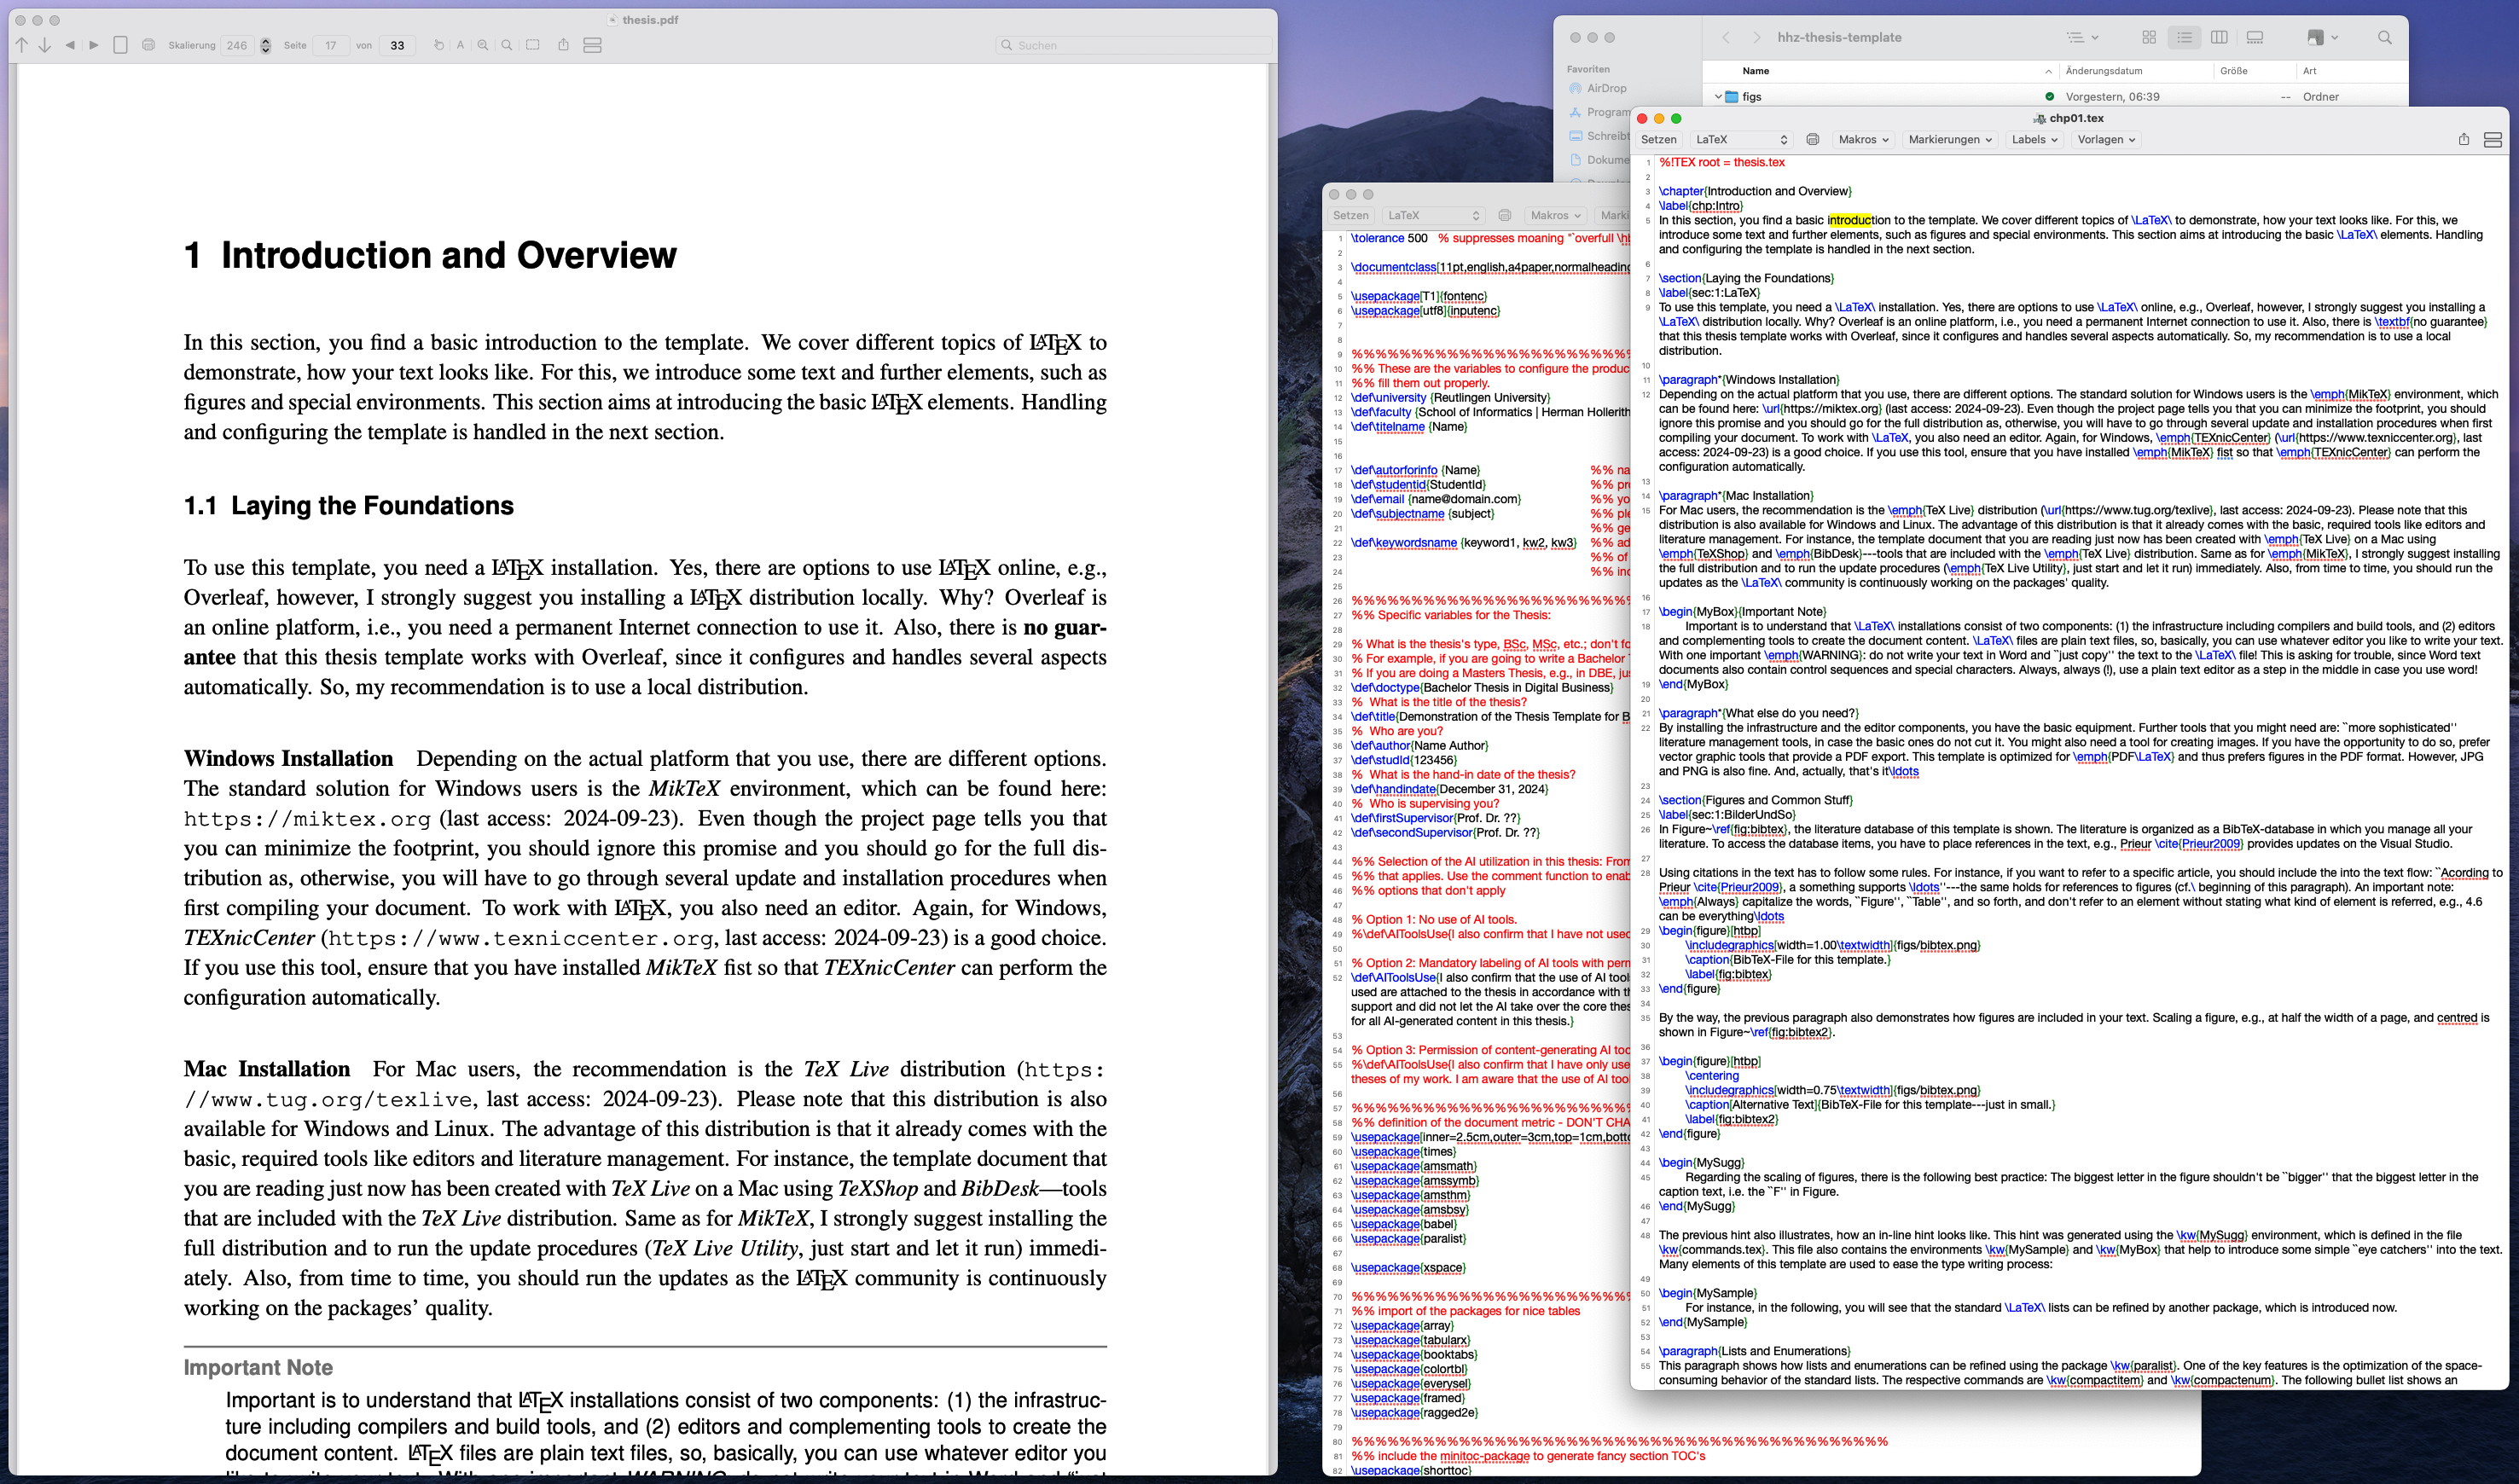
\includegraphics[angle=90, height=0.90\textheight]{figs/latext-edit.png}
	\caption[An example of a \LaTeX\ project in TeXShop from the TeX Live distribution]{An example of a \LaTeX\ project in TeXShop from the TeX Live distribution. This image is also a demonstration of how to rotate pictures in the \kw{includegraphics} command.}
	\label{fig:texshop}
\end{figure}

\begin{MyBox}{Important Note}
	Important is to understand that \LaTeX\ installations consist of two components: (1) the infrastructure including compilers and build tools, and (2) editors and complementing tools to create the document content. \LaTeX\ files are plain text files, so, basically, you can use whatever editor you like to write your text.  With one important \emph{WARNING}: do not write your text in Word and ``just copy'' the text to the \LaTeX\ file! This is asking for trouble, since Word text documents also contain control sequences and special characters. Always, always (!), use a plain text editor as a step in the middle in case you use word!
\end{MyBox}

\paragraph*{What else do you need?}
By installing the infrastructure and the editor components, you have the basic equipment. Further tools that you might need are: ``more sophisticated'' literature management tools, in case the basic ones do not cut it. You might also need a tool for creating images. If you have the opportunity to do so, prefer vector graphic tools that provide a PDF export. This template is optimized for PDF\LaTeX\ and thus prefers figures in the PDF format. However, JPG and PNG is also fine. And, actually, that's it\ldots

\section{Figures and Common Stuff}
\label{sec:1:BilderUndSo}
In Figure~\ref{fig:bibtex}, the literature database of this template is shown. The literature is organized as a BibTeX-database in which you manage all your literature. To access the database items, you have to place references in the text, e.g., Prieur \cite{Prieur2009} provides updates on the Visual Studio. 

Using citations in the text has to follow some rules. For instance, if you want to refer to a specific article, you should include the into the text flow: ``Acording to Prieur \cite{Prieur2009}, a something supports \ldots''---the same holds for references to figures (cf.\ beginning of this paragraph). An important note: \emph{Always} capitalize the words, ``Figure'', ``Table'', and so forth, and don't refer to an element without stating what kind of element is referred, e.g., 4.6 can be everything\ldots
\begin{figure}[htbp]
	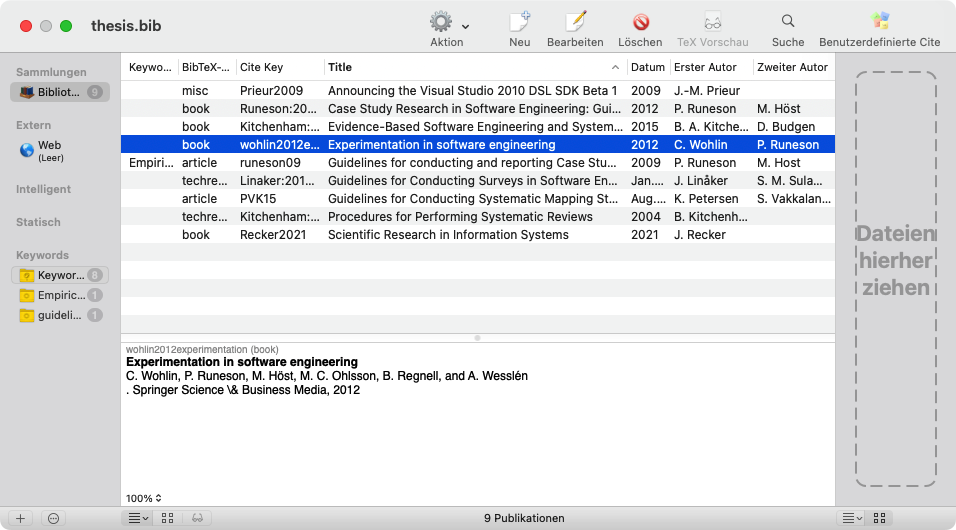
\includegraphics[width=1.00\textwidth]{figs/bibtex.png}
	\caption{BibTeX-File for this template.}
	\label{fig:bibtex}
\end{figure}

By the way, the previous paragraph also demonstrates how figures are included in your text. Scaling a figure, e.g., at half the width of a page, and centred is shown in Figure~\ref{fig:bibtex2}.

\begin{figure}[htbp]
	\centering
	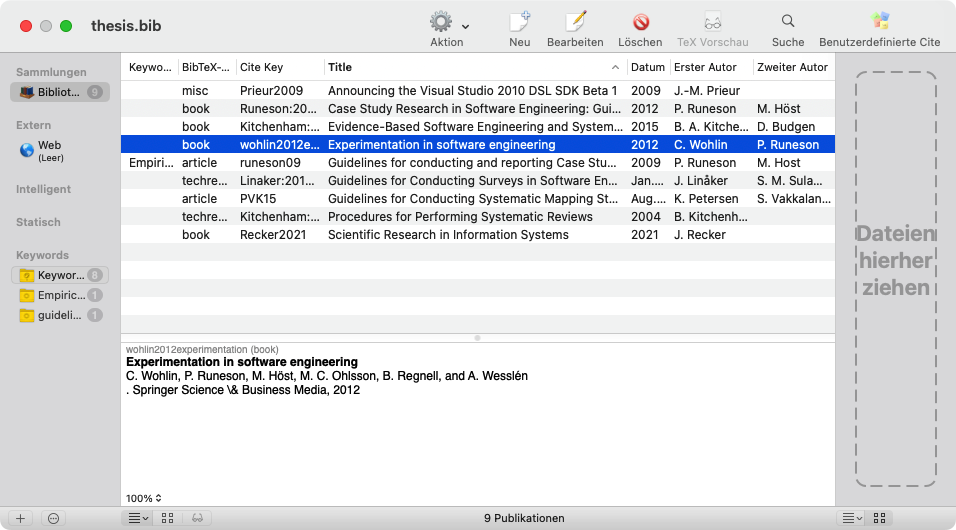
\includegraphics[width=0.75\textwidth]{figs/bibtex.png}
	\caption[Alternative Text]{BibTeX-File for this template---just in small.}
	\label{fig:bibtex2}
\end{figure}

\begin{MySugg}
	Regarding the scaling of figures, there is the following best practice: The biggest letter in the figure shouldn't be ``bigger'' that the biggest letter in the caption text, i.e. the ``F'' in Figure.
\end{MySugg}

The previous hint also illustrates, how an in-line hint looks like. This hint was generated using the \kw{MySugg} environment, which is defined in the file \kw{commands.tex}. This file also contains the environments \kw{MySample} and \kw{MyBox} that help to introduce some simple ``eye catchers'' into the text. Many elements of this template are used to ease the type writing process:

\begin{MySample}
	For instance, in the following, you will see that the standard \LaTeX\ lists can be refined by another package, which is introduced now.
\end{MySample}

\paragraph{Lists and Enumerations}
This paragraph shows how lists and enumerations can be refined using the package \kw{paralist}. One of the key features is the optimization of the space-consuming behavior of the standard lists. The respective commands are \kw{compactitem} and \kw{compactenum}. The following bullet list shows an instance of the ``classic'' \kw{itemize} environment:
\begin{itemize}
	\item Item 1
	\item Item 2
	\item Item 3
\end{itemize}

Using the respective environments from the \kw{paralist} package results in the following output:

\begin{compactitem}
	\item Item 1
	\item Item 2
	\item Item 3
\end{compactitem}

\begin{MySugg}
	Use the paralist-environments if you have to type set only a small list in a key word style. If you use the lists or enumerations for printing more descriptive text, stay with the classic environment to keep paragraph spacing active.
\end{MySugg}


\section{Tables}
\label{sec:Tables}
An important element to structure and to present information is a table. However, the standard tables provided by plain \LaTeX\ are (1) ugly and (2) too inflexible. For this, in this template, we included the package \kw{tabularx} and \kw{booktabs}, which provide rich functionality to configure and present tables properly. \emph{Note:} these packages are quite powerful, but not easy to use---especially if you need tables spanning several pages. Nevertheless, the usual strategies to tackle this are:
\begin{compactenum}
	\item tinkering
	\item having a template
	\item knowing somebody who knows the dark side of the force\ldots
\end{compactenum}
Anyway, in the following, you will find some examples that demonstrate the use of the pre-configured elements of the fancy table environments. Table~\ref{tab:TableReference1} shows an example of an automatically scaled table.
\begin{table}[htbp]
  \caption[Alternative text for table of contents]{Example for a fancy, typographic ``better'' table.}%
  \label{tab:TableReference1}
\begin{tabularx}{\linewidth}{lL}
	\opentableheader  % you can also use \toprule instead
		\hl{Element} & \hl{Description} \\
	\closetableheader % you can also use \midrule, but it looks different...
		Element & Description \\
		Element & Description \\
		\midrule
		Element & Description, Description, Description, Description, Description, Description, Description, Description, Description, Description, Description, Description, Description, Description, Description\ldots \\
	\bottomrule
\end{tabularx}
\end{table}

\begin{table}[!ht]
\begin{center}
  \caption{Example: A non-scaled table}%
  \label{tab:TabNonScaled}
\begin{tabular} {ll}
	\opentableheader  % you can also use \toprule instead
		\hl{Element} & \hl{Description} \\
	\closetableheader % you can also use \midrule, but it looks different...
		Element & Description \\
		Element & Description \\
		\midrule
		Element & Description \\
	\bottomrule
\end{tabular}
\end{center}
\end{table}

In order to support auto-scaling, the template defines some parameters. For instance, the uppercased ``L'' in Table~\ref{tab:TableReference1} (cf.\ Listing~\ref{lst:TableCode}) ensures that the table uses the whole text width (the table is justified with the paper- and text dimensions as defined in the document configuration\footnote{Changing this configuration alters the the behavior of the table configuration as well. By the way, this is an example for inserting a footnote\ldots}). Furthermore, this column-attribute supports automatic line breaks (comparable to the standard \kw{p}-tag).

\begin{lstlisting}[captionpos=b, language=TeX, commentstyle=\color{blue}\itshape, caption=Listing of the table printed above,label=lst:TableCode]
\begin{table}[htbp]
\begin{tabularx}{\linewidth}{lL}
  \opentableheader  % you can also use \toprule instead
	\hl{Element} & \hl{Description} \\
  \closetableheader % you can also use \midrule, but it looks different...
	Element & Description \\
	Element & Description \\
	\midrule
	Element & Description \\
  \bottomrule
\end{tabularx}
  \caption[Alternative text for table of contents]{Example for a fancy, typographic ``better'' table.}%
  \label{tab:TableReference1}
\end{table}
\end{lstlisting}

If scaling Table~\ref{tab:TableReference1} is not necessary, the uppercased ``L'' needs to be replaced by the normal \kw{l}, and the normal \kw{table} can be used instead of the \kw{tabularx} environment. Table~\ref{tab:TabNonScaled} shows the result.

\begin{MySugg}
	In general, you should use tables to present structured information. Also, you should also prefer scaled tables over non-scaled tables. If you have small non-scaled tables, please consider using a list instead. Also, as \LaTeX\ handles the layout usually itself, encourage the tables to be printed on top of the page.
\end{MySugg}

\section{Listings}
\label{sec:2:Listings}
Sometimes it is necessary to include code snippets into your text. For this, the template includes and configures the \kw{listings} package. Listing~\ref{lst:TableCode} shows an example of the usage and the outcome. The file \kw{commands.tex} defines several macros and supporting commands, e.g., to simplify the configuration of programming languages, fonts, and to reset all settings to default.

\begin{MyBox}{A General Recommendation}
	\LaTeX\ was designed to provide a professional and nice looking, harmonic text. Therefore, any changes and adoptions of templates should be done carefully. \LaTeX\ is not Word! Even if the printout of a \LaTeX-generated file looks ``odd'', usually \LaTeX\ is right. Furthermore, this template aims to support the Thesis writing process and, thus, is not intended to provide sophisticated features to create colorful promotion flyers and stuff like that. Instead, the template focusses to improve the standard \LaTeX\ features and to add some elements to simplify the use of \LaTeX\ by, e.g., providing pre-configured environments, macros, and so forth---nothing new is made. Again, \LaTeX\ is not Word and, therefore, you should pay attention to the following points:
	\begin{itemize}
		\item Don't play around with the fonts! The main body text must be type set with a serif font, e.g., Times. Sans serif fonts, e.g., Arial, are for headlines, eye catchers, and screen reading. 
		\item Don't play around with manual spacing, e.g., paragraph separation by forced line breaks. The paragraph separator is---exactly---one (empty) line between two paragraphs.
		\item Wherever possible use floating environments. \LaTeX\ usually cares about meaningful placement. Sometimes this does, however, not work as expected. In such cases, there are means to influence the \LaTeX\ algorithms.
		\item Always explicitly refer to elements and name the elements to which you refer, e.g., ``Table~1.2''---don't use phases like ``the following table'', as \LaTeX\ has sometime own ideas of what ``the following'' really means\ldots
		\item Just follow the way \LaTeX\ proposes to write text.
	\end{itemize}
	In summary, this template provides you with all you need to start writing your Thesis. Concentrate on writing your text and just take the template. \emph{Adjust it only if you really know what you do!}
\end{MyBox}

\section{Language Elements}
\label{sec:LanguageElements}
Which other language elements of \LaTeX\ do I need? Well, actually, if you give the sources of this template a read, you will quite likely finde just everything you need. Of course, depending on the actual context of your work, you might need extra packages and/or specific tools. For using these, check the Internet for respective support.

However, before you start looking around, give the files \kw{commands.tex} and \kw{shortcuts.tex} a read. There are many extra commands, shortcuts, semantic markups, and the like available and ready to use. For instance, if you just want to refer to a method from a program in your text, you can just use the command \kw{method} defined in \kw{shortcuts.tex}. The command ``\kw{\textbackslash method\{Update\}}'' creates the output \kw{Update()}. So, just check, maybe you already find what you need. By the way, if you develop a nice new presentation element, please share it with me so that we can improve the template!

%%% Local Variables: 
%%% mode: latex
%%% TeX-master: "thesis"
%%% End: 